\documentclass{beamer}

\usetheme{metropolis}

\usepackage{sansmath}
\usepackage{listings}
\usepackage{comment}
\usepackage{tikz}
\usetikzlibrary{arrows, positioning, calc}

\title{Zero-Knowledge Proof: Halo 2 for Dummies}
\date{26 November 2022}
\author{Khai Hanh Tang\\ Orochi Network}

\newcommand{\prover}{\mathcal{P}}
\newcommand{\verifier}{\mathcal{V}}
\newcommand{\poly}{\mathsf{poly}}
\newcommand{\polylog}{\mathsf{polylog}}

\newcommand{\wireindices}{\mathcal{I}}

\AtBeginSection[]{
	\begin{frame}
		\vfill
		\centering
		\begin{beamercolorbox}[sep=8pt,center,shadow=false,rounded=true]{title}
			\usebeamerfont{title}\insertsectionhead\par%
		\end{beamercolorbox}
		\vfill
	\end{frame}
}

\begin{document}
	\begin{frame}
		\titlepage
	\end{frame}
	
	\begin{frame}{Outline}
		\tableofcontents
	\end{frame}
	\section{PLONKish Arithmetization}
	\begin{frame}{Zero-Knowledge Proofs / Arguments}
		Proving a statement is true without leaking secret behind.\pause
		
		Properties:\pause
		\begin{itemize}
			\item Completeness\pause
			\item Soundness\pause
			\item Zero Knowledge\pause
		\end{itemize}
	
		zkSNARK: very small proof size.\pause
		\begin{itemize}
			\item Some proofs / arguments have fast verification.
		\end{itemize}
	\end{frame}

	\begin{frame}{Halo 2}
			zkSNARK library in Rust.\pause
			\begin{figure}
				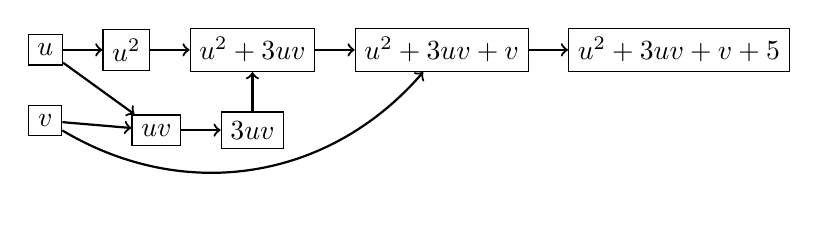
\begin{tikzpicture}[node distance=0.5cm, auto]
					\node [rectangle, draw] (1) {$u^2 + 3uv + v + 5$};
					\node [rectangle, draw, left=of 1] (2) {$u^2 + 3uv + v$};
					\node [rectangle, draw, left = of 2](3){$u^2 + 3uv$};
					\node [rectangle, draw, left = of 3](4){$u^2$};
					\node [rectangle, draw, below = of 3] (5){$3uv$};
					\node [rectangle, draw, left = of 5](6){$uv$};
					\node [rectangle, draw, left = of 4](7){$u$};
					\node [rectangle, draw, below = of 7](8){$v$};
					
					\path[->,draw,thick] 
						(8) edge node[near end]{} (6)
						(7) edge node[near end]{} (6)
						(7) edge node[near end]{} (4)
						(6) edge node[near end]{} (5)
						(5) edge node[near end]{} (3)
						(4) edge node[near end]{} (3)
						(3) edge node[near end]{} (2)
						(8) edge [bend right = 40] node[near end]{} (2)
						(2) edge node[near end]{} (1);
				\end{tikzpicture}
			\end{figure}\pause
			PLONKish arithmetization \footnote{\url{https://zcash.github.io/halo2/concepts/arithmetization.html}}\pause
			\begin{itemize}
				\item built upon PLONK's arithmetization \cite{iacr/GabizonWC19}.\pause
			\end{itemize} 
			
			Compiling arithmetization $\Rightarrow$ zkSNARK.
	\end{frame}

	\begin{frame}{Arithmetization Table for $f(u, v) = u^2 + 3uv + v + 5$ in Halo 2}
		\footnotesize
		\begin{figure}
			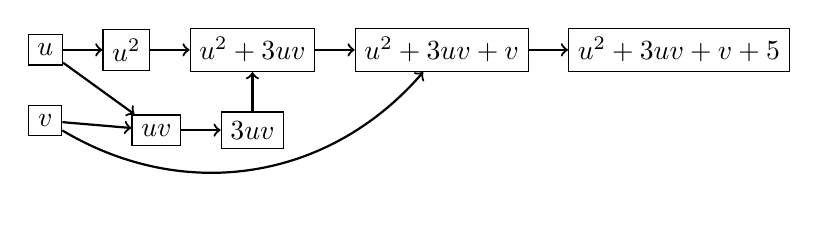
\begin{tikzpicture}[node distance=0.5cm, auto]
				\node [rectangle, draw] (1) {$u^2 + 3uv + v + 5$};
				\node [rectangle, draw, left=of 1] (2) {$u^2 + 3uv + v$};
				\node [rectangle, draw, left = of 2](3){$u^2 + 3uv$};
				\node [rectangle, draw, left = of 3](4){$u^2$};
				\node [rectangle, draw, below = of 3] (5){$3uv$};
				\node [rectangle, draw, left = of 5](6){$uv$};
				\node [rectangle, draw, left = of 4](7){$u$};
				\node [rectangle, draw, below = of 7](8){$v$};
				
				\path[->,draw,thick] 
				(8) edge node[near end]{} (6)
				(7) edge node[near end]{} (6)
				(7) edge node[near end]{} (4)
				(6) edge node[near end]{} (5)
				(5) edge node[near end]{} (3)
				(4) edge node[near end]{} (3)
				(3) edge node[near end]{} (2)
				(8) edge [bend right = 40] node[near end]{} (2)
				(2) edge node[near end]{} (1);
			\end{tikzpicture}
		\end{figure}\pause
		\begin{columns}
			\begin{column}{0.5\textwidth}
				\begin{center}
					\begin{table}
						\scriptsize
						\setlength\tabcolsep{1.5pt}
						\begin{tabular}{|c|c|c|c|c|c|c|c|c|c|}
							\hline
							$\text{adv}_0$&$\text{adv}_1$&$\text{adv}_2$&$\text{const}$&$\text{s}_\text{add}$&$\text{s}_\text{mul}$&$\text{s}_\text{addc}$&$\text{s}_\text{mulc}$\\
							\hline
							$x_{a_1}$&$x_{b_1}$&$x_{c_1}$& & $0$ & $1$ & $0$ & $0$ \\
							$x_{a_2}$&$x_{b_2}$&$x_{c_2}$& & $0$ & $1$ & $0$ & $0$\\
							$x_{a_3}$&&$x_{c_3}$& $3$ & $0$ & $0$ & $0$ & $1$ \\
							$x_{a_4}$&$x_{b_4}$&$x_{c_4}$& & $1$ & $0$ & $0$ & $0$ \\
							$x_{a_5}$&$x_{b_5}$&$x_{c_5}$& & $1$ & $0$ & $0$ & $0$\\
							$x_{a_6}$&&$x_{c_6}$& $5$ & $0$ & $0$ & $1$ & $0$\\
							\hline
						\end{tabular}
					\end{table}\pause
				\end{center}
			\end{column}
			\begin{column}{0.4\textwidth}
					\begin{equation*}
					\begin{cases}
						s_{add} \cdot (\text{adv}_0 + \text{adv}_1 - \text{adv}_2) = 0,\\ 
						s_{mul} \cdot (\text{adv}_0 \cdot \text{adv}_1 - \text{adv}_2) = 0,\\
						s_{addc} \cdot (\text{adv}_0 + \text{const} - \text{adv}_2) = 0,\\ 
						s_{mulc} \cdot (\text{adv}_0 \cdot \text{const} - \text{adv}_2) = 0,\\ 
					\end{cases}
				\end{equation*}
			\end{column}
		\end{columns}\pause
		
		Copy constraints:
		\begin{tabular}{cccc}
			$u = x_{a_1} = x_{a_2} = x_{b_1}$ & $v = x_{b_2} = x_{b_5}$ &$x_{a_4} = x_{c_1}$ & $x_{a_3} = x_{c_2}$\\ 
			$x_{b_4} = x_{c_3}$ & $x_{a_5} = x_{c_4}$ & $x_{a_6} = x_{c_5}$ & $x_{c_6} = f(u,v)$
		\end{tabular}\pause
		
		$f(u, v)$ belongs to instance column.
	\end{frame}
	\section{Implementation in Rust}
	\begin{frame}{Arithmetization Table for $f(u, v) = u^2 + 3uv + v + 5$ in Halo 2}
		\footnotesize
		\begin{figure}
			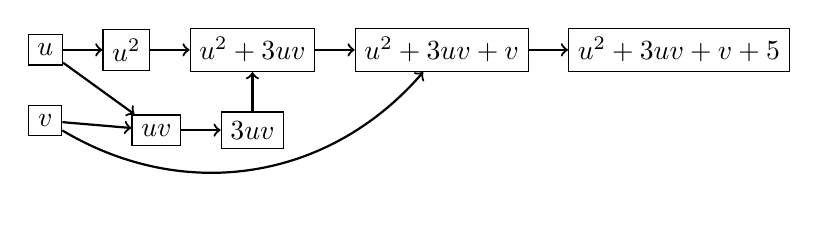
\begin{tikzpicture}[node distance=0.5cm, auto]
				\node [rectangle, draw] (1) {$u^2 + 3uv + v + 5$};
				\node [rectangle, draw, left=of 1] (2) {$u^2 + 3uv + v$};
				\node [rectangle, draw, left = of 2](3){$u^2 + 3uv$};
				\node [rectangle, draw, left = of 3](4){$u^2$};
				\node [rectangle, draw, below = of 3] (5){$3uv$};
				\node [rectangle, draw, left = of 5](6){$uv$};
				\node [rectangle, draw, left = of 4](7){$u$};
				\node [rectangle, draw, below = of 7](8){$v$};
				
				\path[->,draw,thick] 
				(8) edge node[near end]{} (6)
				(7) edge node[near end]{} (6)
				(7) edge node[near end]{} (4)
				(6) edge node[near end]{} (5)
				(5) edge node[near end]{} (3)
				(4) edge node[near end]{} (3)
				(3) edge node[near end]{} (2)
				(8) edge [bend right = 40] node[near end]{} (2)
				(2) edge node[near end]{} (1);
			\end{tikzpicture}
		\end{figure}
		\begin{columns}
			\begin{column}{0.5\textwidth}
				\begin{center}
					\begin{table}
						\scriptsize
						\setlength\tabcolsep{1.5pt}
						\begin{tabular}{|c|c|c|c|c|c|c|c|c|c|c|}
							\hline
							region&$\text{a}_0$&$\text{a}_1$&$\text{a}_2$&$\text{c}$&$\text{s}_\text{add}$&$\text{s}_\text{mul}$&$\text{s}_\text{addc}$&$\text{s}_\text{mulc}$\\
							\hline
							1&$x_{a_1}$&$x_{b_1}$&$x_{c_1}$& & $0$ & $1$ & $0$ & $0$ \\
							&$x_{a_2}$&$x_{b_2}$&$x_{c_2}$& & $0$ & $1$ & $0$ & $0$\\
							&$x_{a_3}$&&$x_{c_3}$& $3$ & $0$ & $0$ & $0$ & $1$ \\
							\hline
							2&$x_{a_4}$&$x_{b_4}$&$x_{c_4}$& & $1$ & $0$ & $0$ & $0$ \\
							&$x_{a_5}$&$x_{b_5}$&$x_{c_5}$& & $1$ & $0$ & $0$ & $0$\\
							&$x_{a_6}$&&$x_{c_6}$& $5$ & $0$ & $0$ & $1$ & $0$\\
							\hline
						\end{tabular}
					\end{table}
				\end{center}
			\end{column}
			\begin{column}{0.4\textwidth}
				\begin{equation*}
					\begin{cases}
						s_{add} \cdot (\text{adv}_0 + \text{adv}_1 - \text{adv}_2) = 0,\\ 
						s_{mul} \cdot (\text{adv}_0 \cdot \text{adv}_1 - \text{adv}_2) = 0,\\
						s_{addc} \cdot (\text{adv}_0 + \text{const} - \text{adv}_2) = 0,\\ 
						s_{mulc} \cdot (\text{adv}_0 \cdot \text{const} - \text{adv}_2) = 0,\\ 
					\end{cases}
				\end{equation*}
			\end{column}
		\end{columns}
		
		Copy constraints:
		\begin{tabular}{cccc}
			$u = x_{a_1} = x_{a_2} = x_{b_1}$ & $v = x_{b_2} = x_{b_5}$ &$x_{a_4} = x_{c_1}$ & $x_{a_3} = x_{c_2}$\\ 
			$x_{b_4} = x_{c_3}$ & $x_{a_5} = x_{c_4}$ & $x_{a_6} = x_{c_5}$ & $x_{c_6} = f(u,v)$
		\end{tabular}
		
		$f(u, v)$ belongs to instance column.
	\end{frame}
	\begin{comment}
	\section{Circuit Specification}
	\begin{frame}{Problem Statement}
		Let $\mathcal{C}$ be a program computing a function, e.g., $$f(u, v) = u^2 + 3uv + v + 5.$$
		Construct a zkSNARK for satisfaction of 
		\begin{equation*}
			\mathcal{C}(\mathbf{x}) = \mathbf{y}
		\end{equation*}
		where $\mathbf{x}$ is private while $\mathcal{C}$ and $\mathbf{y}$ are public.
	\end{frame}

	\begin{frame}{Overview of Arithmetization}
		Arithmetization: transforming program to a form that can be compiled into zk proofs.
		
		Other intuition: representing such program in some language.
		
		This talk: 
		\begin{itemize}
			\item PLONK's arithmetization \cite{iacr/GabizonWC19} and 
			\item Halo 2's PLONKish \footnote{\url{https://zcash.github.io/halo2/concepts/arithmetization.html}}.
		\end{itemize}
	\end{frame}

	\begin{frame}{Circuit Specification}
		Let $\mathcal{C}$ be a circuit of $n$ gates, including:
		\begin{itemize}
			\item Additions,
			\item Multiplications,
			\item Additions with constants, and 
			\item Multiplications with constants.
		\end{itemize}
		Computations are in some finite field $\mathbb{F}$.
		
		Intuition about $\mathbb{F}$:
		\begin{itemize}
			\item Can compute additions, subtractions, multiplications.
			\item Can compute divisions w.r.t non-zero divisors.
			\item Examples: $\mathbb{Z}_3 = \{0, 1, 2\}$, $\mathbb{Z}_7 = \{0, 1, 2, 3, 4, 5, 6\}$.
		\end{itemize}
	\end{frame}

	\begin{frame}{Example}
		Computing $f(u, v) = u^2 + 3uv + v + 5$ in finite field $\mathbb{F}$. 
		
		 Circuit specification:
		 \begin{equation*}
		 	\begin{cases}
		 		t_1 = u \cdot u,&\text{(multiplication)}\\
		 		t_2 = u \cdot v,&\text{(multiplication)}\\
		 		t_3 = t_2 \cdot 3,&\text{(multiplication with constant)}\\
		 		t_4 = t_1 + t_3,&\text{(addition)}\\
		 		t_5 = t_4 + v,&\text{(addition)}\\
		 		t_6 = t_5 + 5.&\text{(addition with constant)}
		 	\end{cases}
		 \end{equation*}
	\end{frame}

	\section{PLONK's Arithmetization}
	\begin{frame}{Labeling circuit wires with selectors}
		Let $x : \{a_1, \dots, a_n, b_1, \dots, b_n, c_1, \dots, c_n\} \rightarrow \mathbb{F}$.
		
		Intuition: view $x$ as an array whose indices are $a_1, \dots, c_n$.
		
		For each gate $i \in [n]$, represent with the form
		\begin{equation*}
			(q_L)_i \cdot x_{a_i} + (q_R)_i \cdot x_{b_i} + (q_O)_i \cdot x_{c_i} + (q_M)_i \cdot (x_{a_i} \cdot x_{b_i}) + (q_C)_i = 0.
		\end{equation*}
		
		$(q_L)_i, (q_R)_i, (q_O)_i, (q_M)_i, (q_C)_i$: selectors determined by the gate.
		
		In particular,
		\begin{itemize}
			\item Addition: $(q_L)_i = 1, (q_R)_i = 1, (q_O)_i = -1, (q_M)_i = 0, (q_C)_i = 0$.
			\item Multiplication: $(q_L)_i = 0, (q_R)_i = 0, (q_O)_i = -1, (q_M)_i = 1, (q_C)_i = 0$.
		\end{itemize}
	\end{frame}

	\begin{frame}{Example}
		Label wires of each gate separately as follows:
		\begin{equation*}
			\begin{cases}
				t_1 = u \cdot u,\\
				t_2 = u \cdot v,\\
				t_3 = t_2 \cdot 3,\\
				t_4 = t_1 + t_3,\\
				t_5 = t_4 + v,\\
				t_6 = t_5 + 5.
			\end{cases}
			\Rightarrow
			\begin{cases}
				x_{c_1} = x_{a_1} \cdot x_{b_1},\\
				x_{c_2} = x_{a_2} \cdot x_{b_2},\\
				x_{c_3} = x_{a_3} \cdot 3,\\
				x_{c_4} = x_{a_4} + x_{b_4},\\
				x_{c_5} = x_{a_5} + x_{b_5},\\
				x_{c_6} = x_{a_6} + 5.
			\end{cases}
		\end{equation*}
	
		Putting selectors:
		\begin{equation*}
			\begin{cases}
				0 \cdot x_{a_1} + 0 \cdot x_{b_1} + (-1) \cdot x_{c_1} + 1 \cdot (x_{a_1}\cdot x_{b_1}) + 0 = 0,\\
				\qquad\qquad\qquad\qquad\qquad\vdots \\
				1 \cdot x_{a_6} + 0 \cdot x_{b_6} + (-1) \cdot x_{c_6} + 0 \cdot (x_{a_6}\cdot x_{b_6}) + 5 = 0.
			\end{cases}
		\end{equation*}
	\end{frame}

	\begin{frame}{Copy constraints}
		\begin{equation*}
			\begin{cases}
				t_1 = u \cdot u,\\
				t_2 = u \cdot v,\\
				t_3 = t_2 \cdot 3,\\
				t_4 = t_1 + t_3,\\
				t_5 = t_4 + v,\\
				t_6 = t_5 + 5.
			\end{cases}\Rightarrow
			\begin{cases}
				x_{c_1} = x_{a_1} \cdot x_{b_1},\\
				x_{c_2} = x_{a_2} \cdot x_{b_2},\\
				x_{c_3} = x_{a_3} \cdot 3,\\
				x_{c_4} = x_{a_4} + x_{b_4},\\
				x_{c_5} = x_{a_5} + x_{b_5},\\
				x_{c_6} = x_{a_6} + 5.
			\end{cases}
		\end{equation*}
	
		Additional requirements (copy constraints):
		\begin{itemize}
			\item $x = x_{a_1} = x_{b_1} = x_{a_2}$,\\
			\item $t_1 = x_{c_1} = x_{a_4}$,\\
			\item \dots
		\end{itemize}
		$\Rightarrow$ checking using permutation argument.
	\end{frame}
	\begin{frame}{Checking copy constraints}
		Let $\{i_1, \dots, i_k\} \subseteq \{a_1, \dots, a_n, b_1, \dots, b_n, c_1, \dots, c_n\}$ s.t 
		\begin{equation*}
			\begin{cases}
				i_1 < i_2 < \dots < i_k \\
				x_{i_1} = x_{i_2} = \dots = x_{i_k}
			\end{cases}
		\end{equation*}
		
		Observation: 
		\begin{equation*}
			\mathbf{a} = \left((i_1, x_{i_1}), \dots, (i_k, x_{i_k})\right) 
		\end{equation*}
		is a permutation of 
		\begin{equation*}
			\mathbf{b} = \left((i_k, x_{i_1}), (i_1, x_{i_2}), \dots, (i_{k - 1}, x_{i_k})\right) 
		\end{equation*}
		if and only if 
		\begin{equation*}
			x_{i_1} = x_{i_2} = \dots = x_{i_k}
		\end{equation*}
	
		``$\Leftarrow$'' direction is trivial.
	\end{frame}
	\begin{frame}{Proof of ``$\Rightarrow$''}
		Assume that 
			\begin{equation*}
			\mathbf{a} = \left((i_1, x_{i_1}), \dots, (i_k, x_{i_k})\right)
		\end{equation*}
		is a permutation of 
		\begin{equation*}
			\mathbf{b} = \left((i_k, x_{i_1}), (i_1, x_{i_2}), \dots, (i_{k - 1}, x_{i_k})\right).
		\end{equation*}
	
		Since $i_1, \dots, i_k$ are distinct, we have
		\begin{equation*}
			(i_j, x_{i_j}) = (i_j, x_{i_{(j \mod k + 1)}})
		\end{equation*}
		where LHS and RHS are from $\mathbf{a}$ and $\mathbf{b}$, respectively.
		
		Hence $x_{i_1} = \dots = x_{i_{(j \mod k + 1)}}$.
	\end{frame}
	\begin{frame}{Final PLONK's Arithmetization}
		\begin{itemize}
			\item Relabel with selectors. Prove correct evaluation with selectors.
			\item Guaranteeing equality among wires (copy constraints).
		\end{itemize}
	\end{frame}
	\begin{comment}
	\begin{frame}{Example}
		$$\begin{cases}
				u = x_{a_1} = x_{a_2} = x_{b_1},\\
				v = x_{b_2} = x_{b_5},\\
				t_1 = x_{a_4} = x_{c_1},\\
				t_2 = x_{a_3} = x_{c_2},\\
				t_3 = x_{b_4} = x_{c_3},\\
				t_4 = x_{a_5} = x_{c_4},\\
				t_5 = x_{a_6} = x_{c_5},\\
				t_6 = x_{c_6}.
			\end{cases} \Rightarrow \begin{cases}
				\sigma(a_1) = b_1,\quad \sigma(a_2) = a_1, \quad\sigma(b_1) = a_2,\\
				\sigma(b_2) = b_5, \quad \sigma(b_5) = b_2,\\
				\sigma(a_4) = c_1, \quad\sigma(c_1) = a_4,\\
				\sigma(a_3) = c_2, \quad\sigma(c_2) = a_3,\\
				\sigma(b_4) = c_3, \quad\sigma(c_3) = b_4,\\
				\sigma(a_5) = c_4, \quad\sigma(c_4) = a_5,\\
				\sigma(a_6) = c_5, \quad\sigma(c_5) = a_6,\\
				\sigma(c_6) = c_6.
			\end{cases}$$
	\end{frame}
	\section{PLONKish Arithmetization}
	\begin{frame}{Overview of PLONKish Arithmetization}
		Support custom gates.
		
		Configuration \footnote{\url{https://zcash.github.io/halo2/concepts/arithmetization.html}}:
		\begin{itemize}
			\item Finite field $\mathbb{F}$.
			\item Columns: Fixed, Instance, Advice and Selectors.
			\item Copy constraints and columns for copy constraints.
			\item Maximum constraint degree.
			\item Polynomial constraints.
			
		\end{itemize}
	\end{frame}

	\begin{frame}{More on Custom Gates}
		PLONK's Arithmetization:
		$$
			(q_L)_i \cdot x_{a_i} + (q_R)_i \cdot x_{b_i} + (q_O)_i \cdot x_{c_i} + (q_M)_i \cdot (x_{a_i} \cdot x_{b_i}) + (q_C)_i = 0.
		$$
		
		PLONKish's Arithmetization:
		\begin{itemize}
			\item $h$ selectors $s_{i_1}, \dots, s_{i_h}$ for each row;
			\item $k$ variables $x_{i_1}, \dots, x_{i_h}$ for each row;
			\item $m$ gates represented by $g_1(s_{i_1}, \dots, s_{i_h}, x_{i_1}, \dots, x_{i_h}), \dots, g_m(s_{i_1}, \dots, s_{i_h}, x_{i_1}, \dots, x_{i_k})$;
			\item Equation
			$$
				\sum_{g = 1}^m g_j(s_{i_1}, \dots, s_{i_h}, x_{i_1}, \dots, x_{i_k}) = 0.
			$$ 
		\end{itemize}
	\end{frame}


	\section{An Example Implementation from Halo 2}
	\end{comment}
	

	\begin{frame}{}
		\begin{center}
			{\fontsize{20}{20}\selectfont Thank You!}
		\end{center}
	\end{frame}

	\begin{frame}[allowframebreaks]{References}
		\setbeamertemplate{bibliography item}[text]
		\bibliographystyle{alpha}
		\bibliography{refs.bib}
		
	\end{frame}
	
\end{document}